\section{Durchführung als Projekt}
\subsection{Ziele}
\steffen
Ziel der Unterrichtsreihe ist es, die Schüler den mathematischen Modellierungskreislauf herleiten und durchführen zu lassen. Als Modellierungsobjekt dient dabei die Modellierung von Epidemien und Pandemien. 


\begin{landscape}
\subsection{Reihenplanung}
\noindent
\begin{longtable}{|C{0.05\textwidth}|L{0.2\textwidth}|L{0.3\textwidth}|L{0.25\textwidth}|L{0.3\textwidth}|L{0.25\textwidth}|L{0.1\textwidth}|}
\hline
Std&Inhalte&Grobziele \& Kompetenzen&Wdh \& Festigung&didakt. \& method. Auswahl&Medien&Sonstiges\\
\hline\hline
\endhead
\hline
\endfoot
1\&{}2 &\emph{SIHDR}&\begin{itemize}
	\item Schüler durchlaufen den Modellierungskreislauf zwei mal
	\item K2
	\item K3
\end{itemize}&--&\begin{itemize}
	\item Modell von \emph{SID} zu \emph{SIHDR}
	\item TPS zur Modellbildung
	\item Zwischenergebnisse werden in der Klasse besprochen
	\item Durch Aufgabenstellung wenig Varianz in Modellierung
\end{itemize}&\begin{itemize}
	\item Ta\-bel\-len\-kal\-ku\-la\-tion
\end{itemize}&--\\\hline
3\&{}4&\begin{itemize}
	\item Mo\-del\-lier\-ungs\-kreis\-lauf
	\item \emph{SIHFDR}
\end{itemize}&b&c&d&e&f\\\hline
5\&{}6&\begin{itemize}
	\item Maß\-nahmen gegen Ausbreitung
	\item Schwächen des Modells
	\item Erwei\-terung auf mehrere Nationen
\end{itemize}&\begin{itemize}
	\item K2
	\item K3
\end{itemize}&Model der Vorstunde&d&e&f\\
\end{longtable}
\end{landscape}
\subsection{Projektstunde 1 \& 2}\ellen
\subsubsection{Bemerkungen zur Lerngruppe}
Bei der Planung der ersten beiden Stunden war uns lediglich bekannt, dass es sich um Schülerinnen und Schüler der zehnten Klasse eines Gymnasiums für Hochbegabte handelt\\
Zudem seien die Grundlagen der Schülerinnen und Schüler höchst unterschiedlich. Der Umgang mit Tabellenkalkulationsprogrammen sollte jedoch in Grundzügen beherrscht werden. 
\subsubsection{Methodische Überlegungen}
Um die Motivation zu fördern und eine möglichst hohe Nachhaltigkeit zu erhalten, sollen die Unterrichtsstunden handlungsorientiert ausgerichtet werden. Dazu sollen die Schülerinnen und Schüler zunächst alleine Rechenoperationen formulieren, mit deren Hilfe die Größe der Klassen (Gesund, Krank und Tod) berechnet werden können.\\
Die Schülerinnen und Schüler haben bereits vorher im Mathematikunterricht gelernt, wie sie aus Texten Terme aufstellt. Dadurch können die Schülerinnen und Schüler früh Erfolge erringen um dadurch die Motivation zu behalten und um ihnen die Angst vor dem Simulieren nehmen.\\
Durch die Einzelarbeit ist gewährleistet, dass alle Schülerinnen und Schüler sich am Unterricht beteiligen. Sobald alle Schülerinnen und Schüler ihre Terme aufgestellt haben, vergleichen sie ihre mit denen ihres Nachbarn.\\
Dadurch können die Schülerinnen und Schüler mathematisches argumentieren einüben. Zusätzlich entsteht eine gewisse Sicherheit bezüglich des eigenen Vorgehens, dadurch kann die Hemmschwelle gesenkt werden, die eigenen Ergebnisse der Klasse vorzustellen.\\
Nachdem sich alle Gruppen auf Vorschriften geeinigt haben, werden diese der Klasse vorgestellt.\\
In der Klasse werden die Vorschriften vorgestellt. Dabei sollten falsche Vorschriften nicht direkt durch die Lehrperson korrigiert werden. Die Schülerinnen und Schüler können später über die Gleichungen diskutieren und gemeinsam eine korrekte Lösung erarbeiten.\\
Mit diesen Vorschriften sollen die Schülerinnen und Schüler dann eine kleine Simulation mit Hilfe von Tabellenkalkulationsprogrammen erstellen.\\
Der Umgang mit solchen Programmen sollte in Grundzügen bereits beherrscht werden und wird an dieser Stelle vertieft.\\
Nachdem diese Programme angefertigt und in der Klasse besprochen wurden, sollen die Schülerinnen und Schüler Vorschläge zur Verbesserung des Modells machen. Manche dieser Vorschläge werden dann in einem zweiten Programm umgesetzt.\\
Dadurch haben die Schülerinnen und Schüler den Modellierungskreislauf durchgeführt. 
%\subsubsection{Verlaufsskizze}
\begin{landscape}
\subsubsection{Verlaufsskizze}
\noindent
\begin{tabular}{|C{0.3\textwidth}|L{0.8\textwidth}|L{0.4\textwidth}|}
\hline
Phase & Arbeitsauftrag & Sozialform\\
\hline\hline
Begrüßung & keine & Lehrervortrag\\
\hline
Einstieg & Lesen der Informationen über Ebola & Einzelarbeit\\
\hline
1. Erarbeitungsphase (a) & Modell entwickeln zur Simulation einer Ebola Epidemie & Einzelarbeit\\
\hline
1. Erarbeitungsphase (b) & Modell mit dem Nachbarn vergleichen, ein gemeinsames Modell erarbeiten & Partnerarbeit\\
\hline
1. Erarbeitungsphase (c) & Das gemeinsame Modell mit Hilfe von Tabellenkalkulationsprogramm simulieren & Partnerarbeit\\
\hline
1. Reflexionsphase & Modelle der SuS werden vorgestellt und Stärken und Schwächen der Modelle besprochen & Schülervorträge + Diskussion\\
\hline
2. Erarbeitungsphase & Mit neuen Informationen und den Überlegungen aus der Diskussion wird das Modell verbessert und wieder eine Simulation durchgeführt & Partnerarbeit\\
\hline
\end{tabular}
\end{landscape}
\subsubsection{Materialien}
\noindent\frame{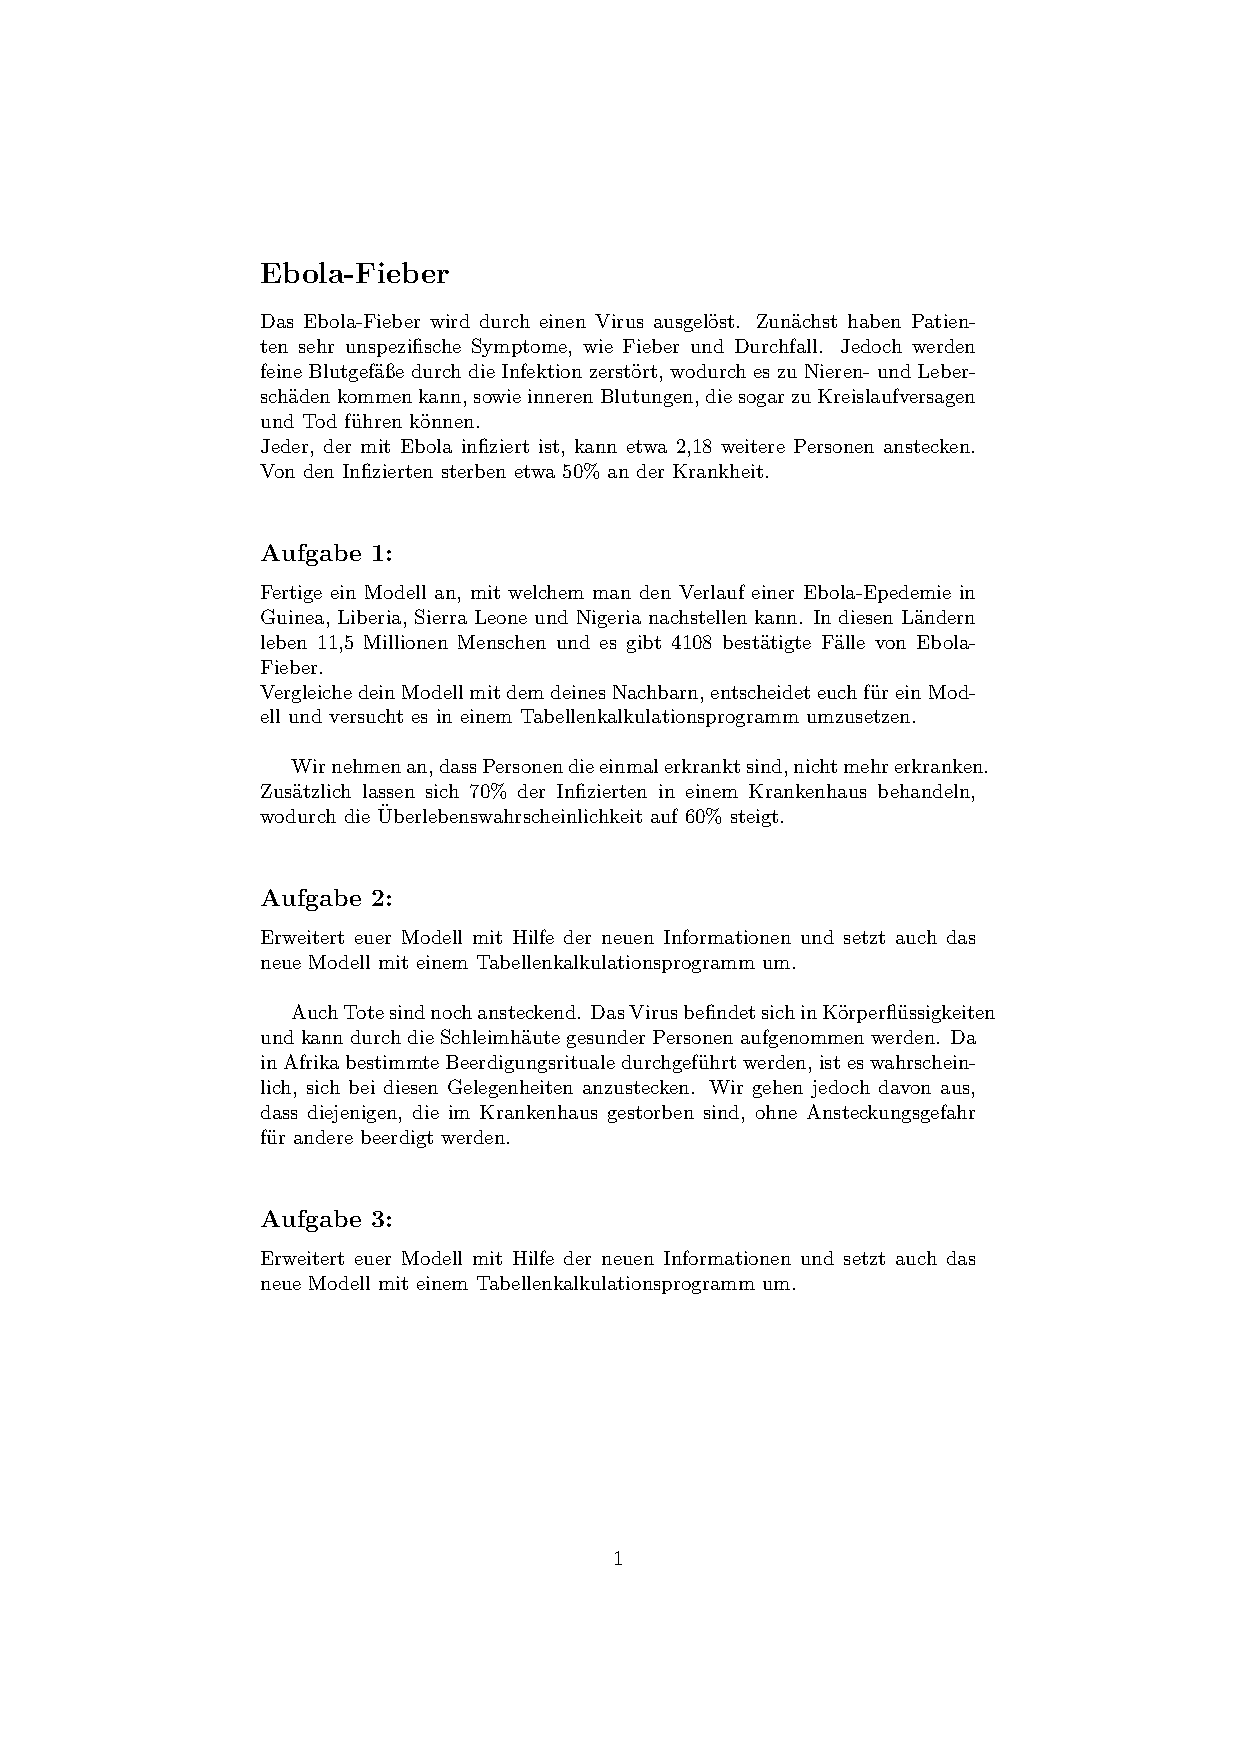
\includegraphics[width=\textwidth]{projekt/Arbeitsblatt_1}}
\subsubsection{Erwartungshorizont}
Da die Schülerinnen und Schüler bereits gelernt haben, wie sie Gleichungen aufstellen wird erwartet, dass sie zunächst einige Schritte ausprobieren und danach eine Vorschrift für eine beliebige Zeit angeben. Dies könnte dann etwa so aussehen:\\
Zunächst sollten die Kranken betrachtet werden, da diese lediglich von der Anzahl der Kranken zuvor abhängt.\\
$ K(1) = K$\\
$ K(2) = 2,18 \cdot K(1) - K(1) = 1,18 \cdot K(1)$\\
$ K(3) = 1,18 \cdot K(2) = 1,18^2 \cdot K(1)$\\
$ K(t) = 1,18^{t-1} \cdot K(1)$\\

Danach können sie eine Vorschrift für die Gesunden mit der gleichen Vorgehensweise finden.\\
$ G(1) = G$\\
$ G(2) = G(1) - 2,18 \cdot K(1) + 0,5 \cdot K(1) = G(1)- 1,68 \cdot K(1)$\\
$ G(3) = G(2) - 1,68 \cdot K(2)$\\
$ G(t) = G(t-1) - 1,68 \cdot K(t-1)$\\
Diese Gleichung kann selbstverständlich auch anders formuliert werden und explizit dargestellt werden. Diese Darstellung lässt sich jedoch leicht mit Tabellenkalkulationsprogrammen durch ziehen der Formeln umsetzen.\\

Ebenso sollen die Schülerinnen und Schüler Vorschriften für die Anzahl der Toten angeben.\\
$ T(1) = 0 $\\
$ T(t) = T(t-1) + 0,5 \cdot K(t-1)$\\


\noindent\frame{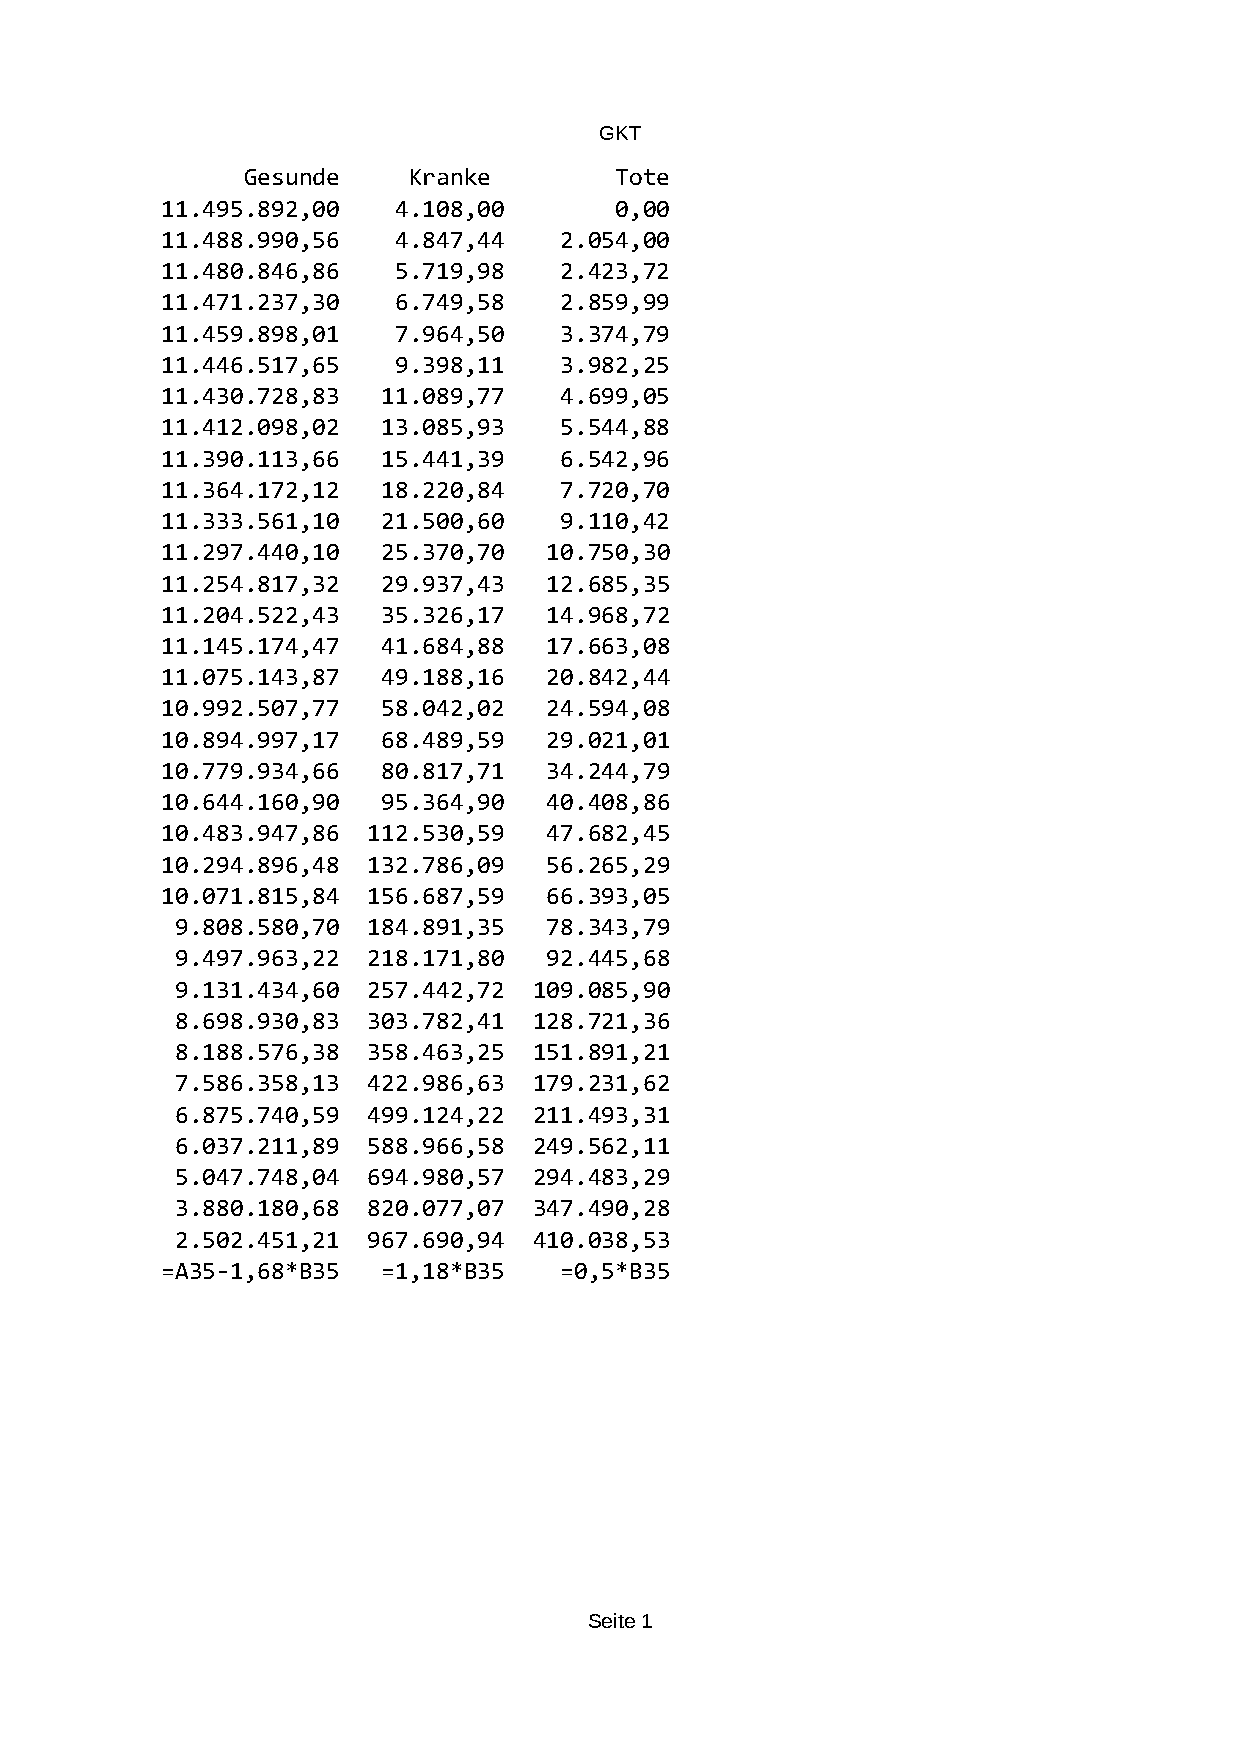
\includegraphics[width=\textwidth]{projekt/erwartung_gtk}}\newpage
\noindent\frame{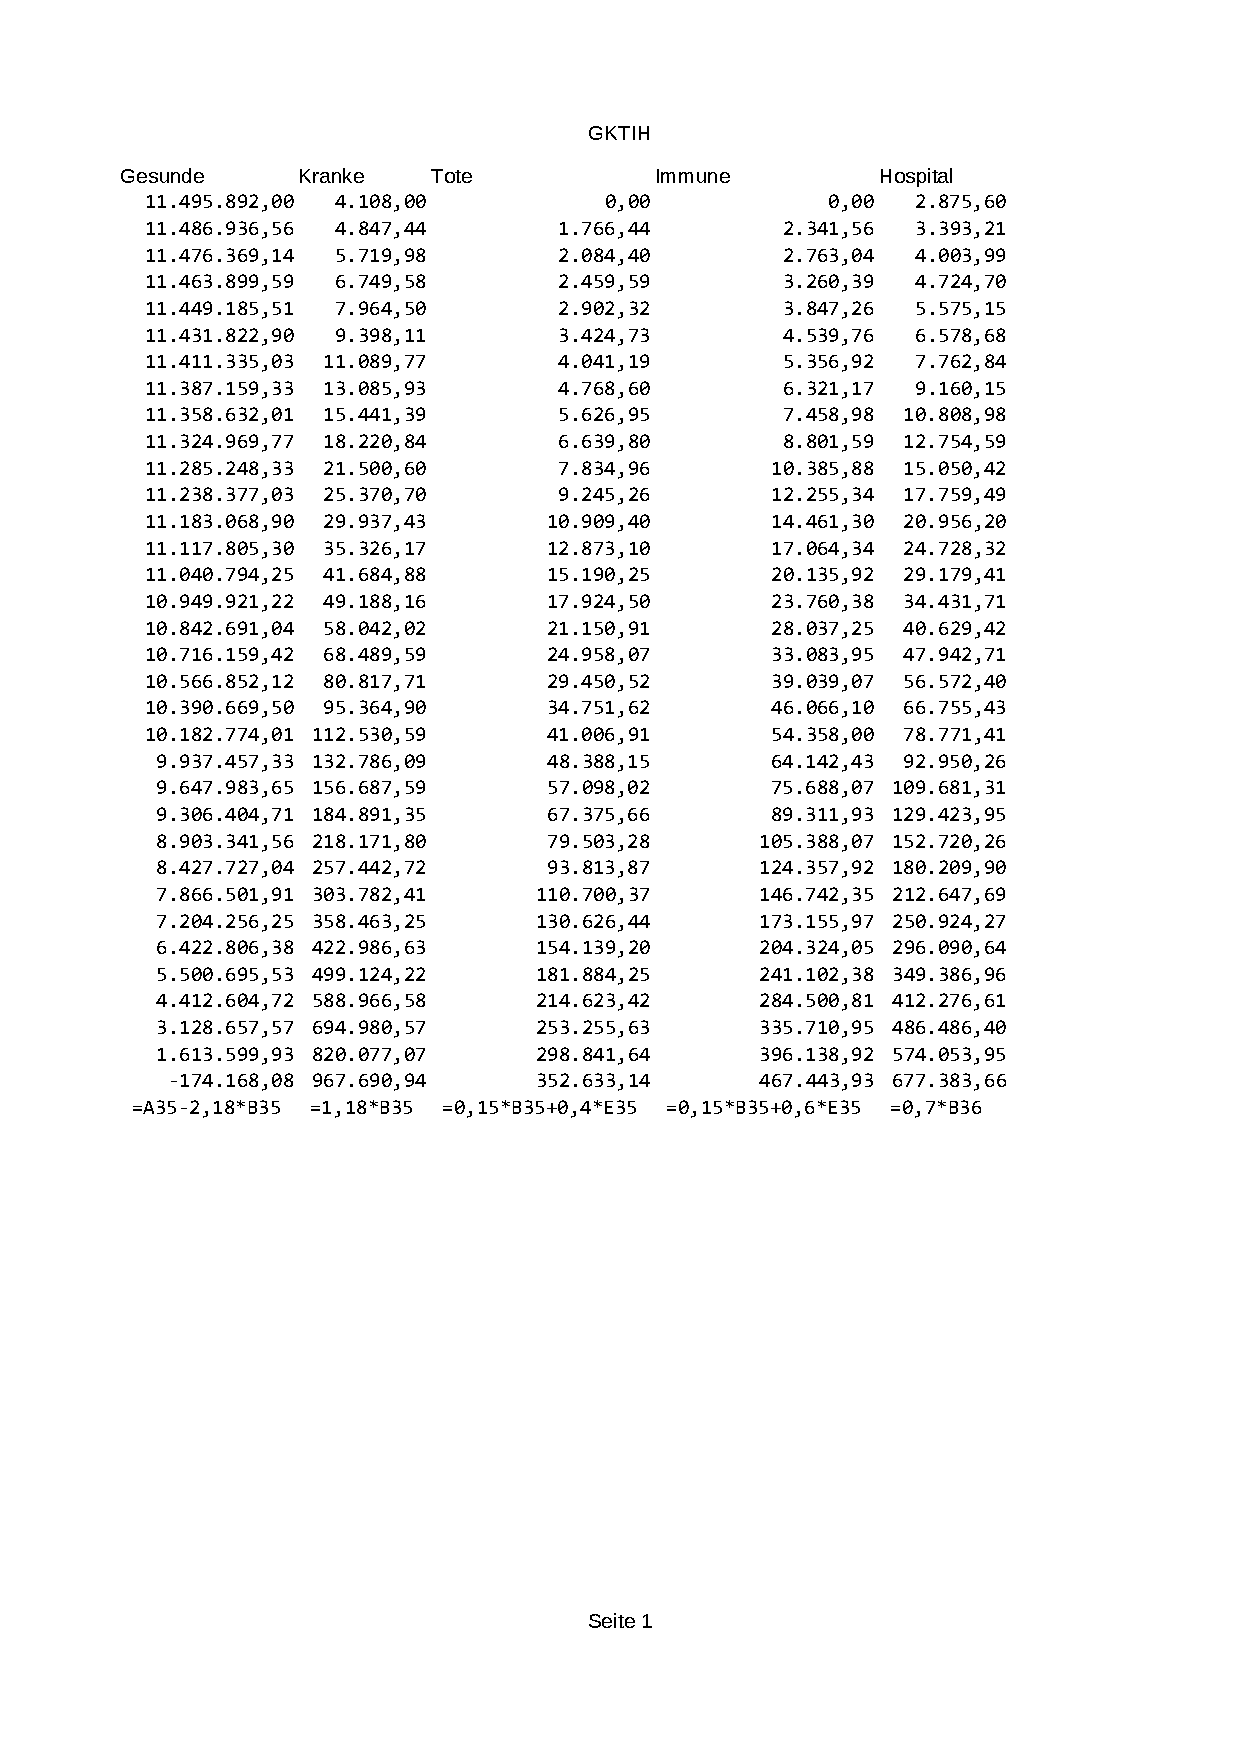
\includegraphics[width=\textwidth]{projekt/erwartung_gtih}}\newpage
\noindent\frame{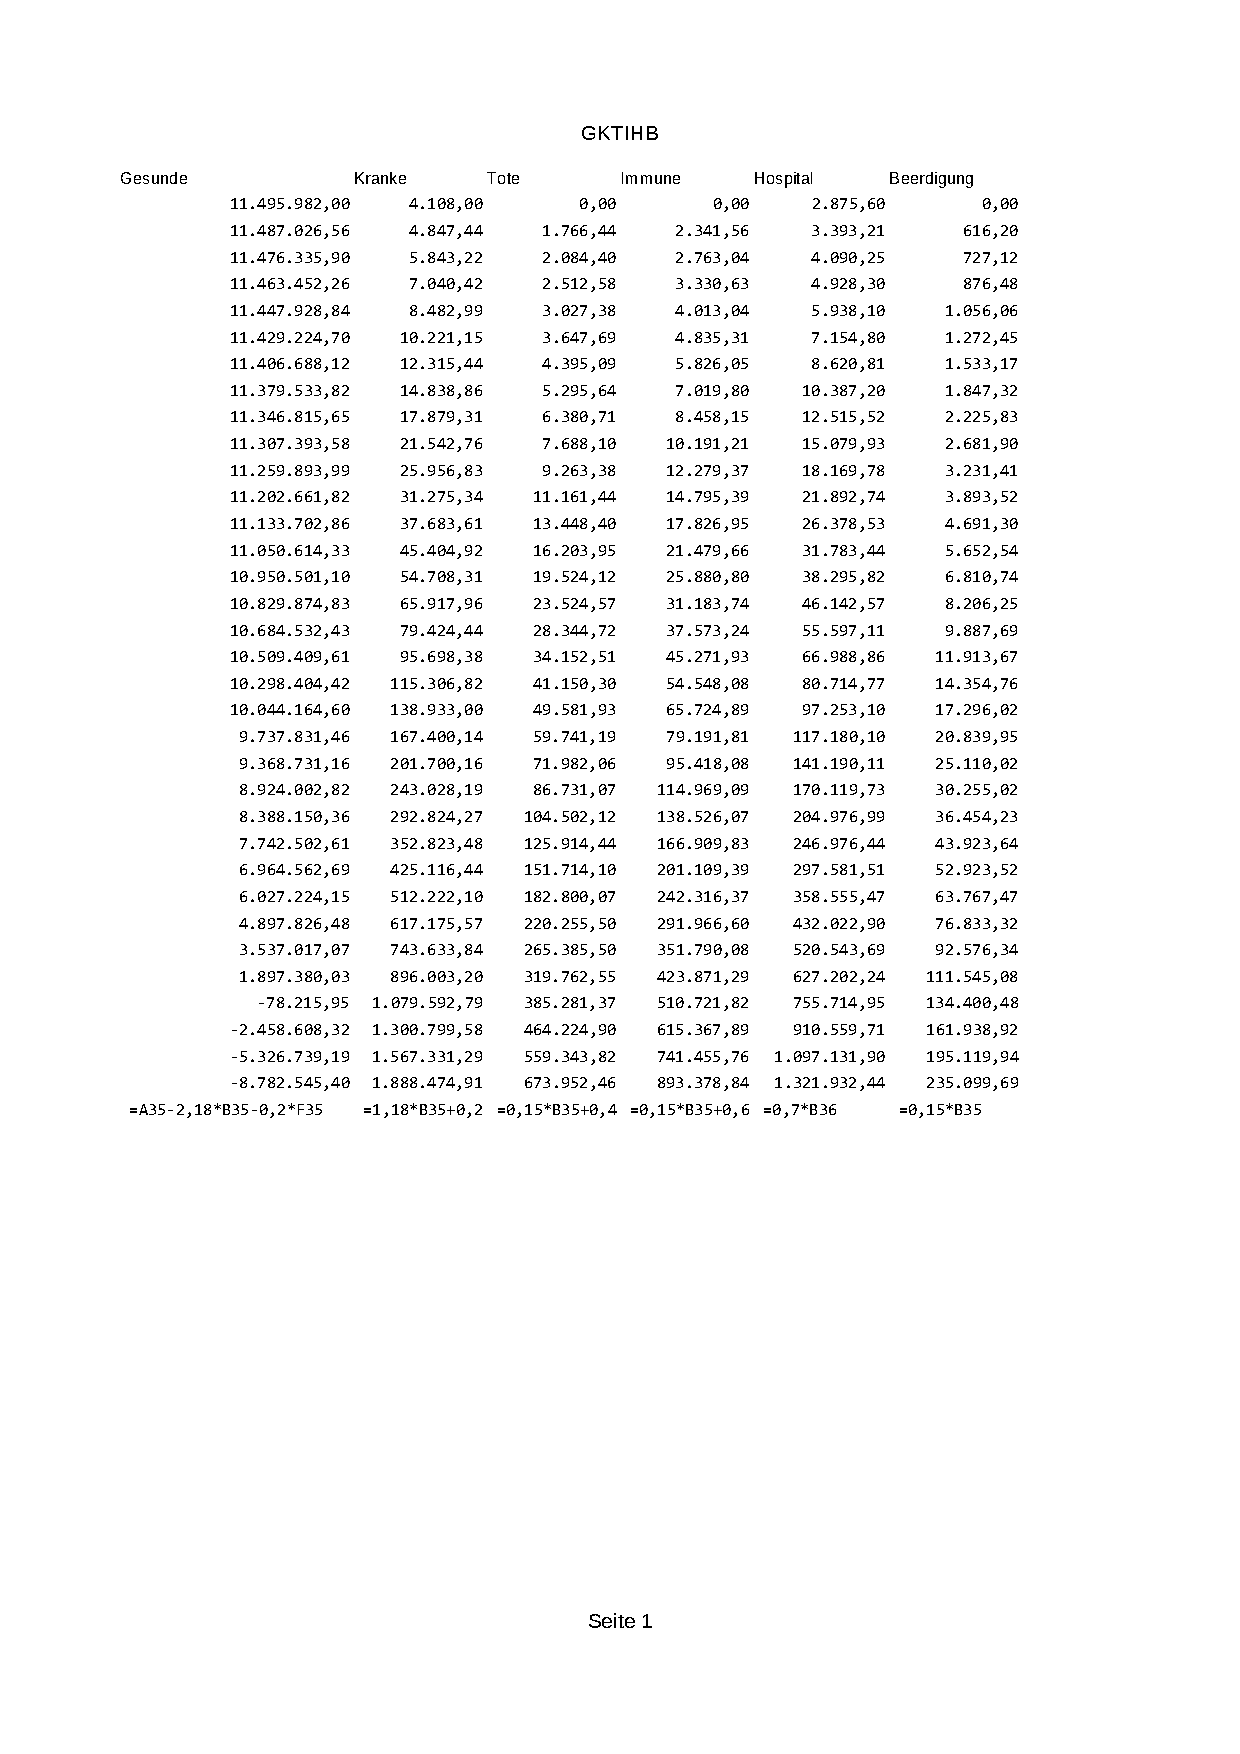
\includegraphics[width=\textwidth]{projekt/erwartung_gktihb}}\newpage
\subsubsection{Schülerprodukte}
\noindent\frame{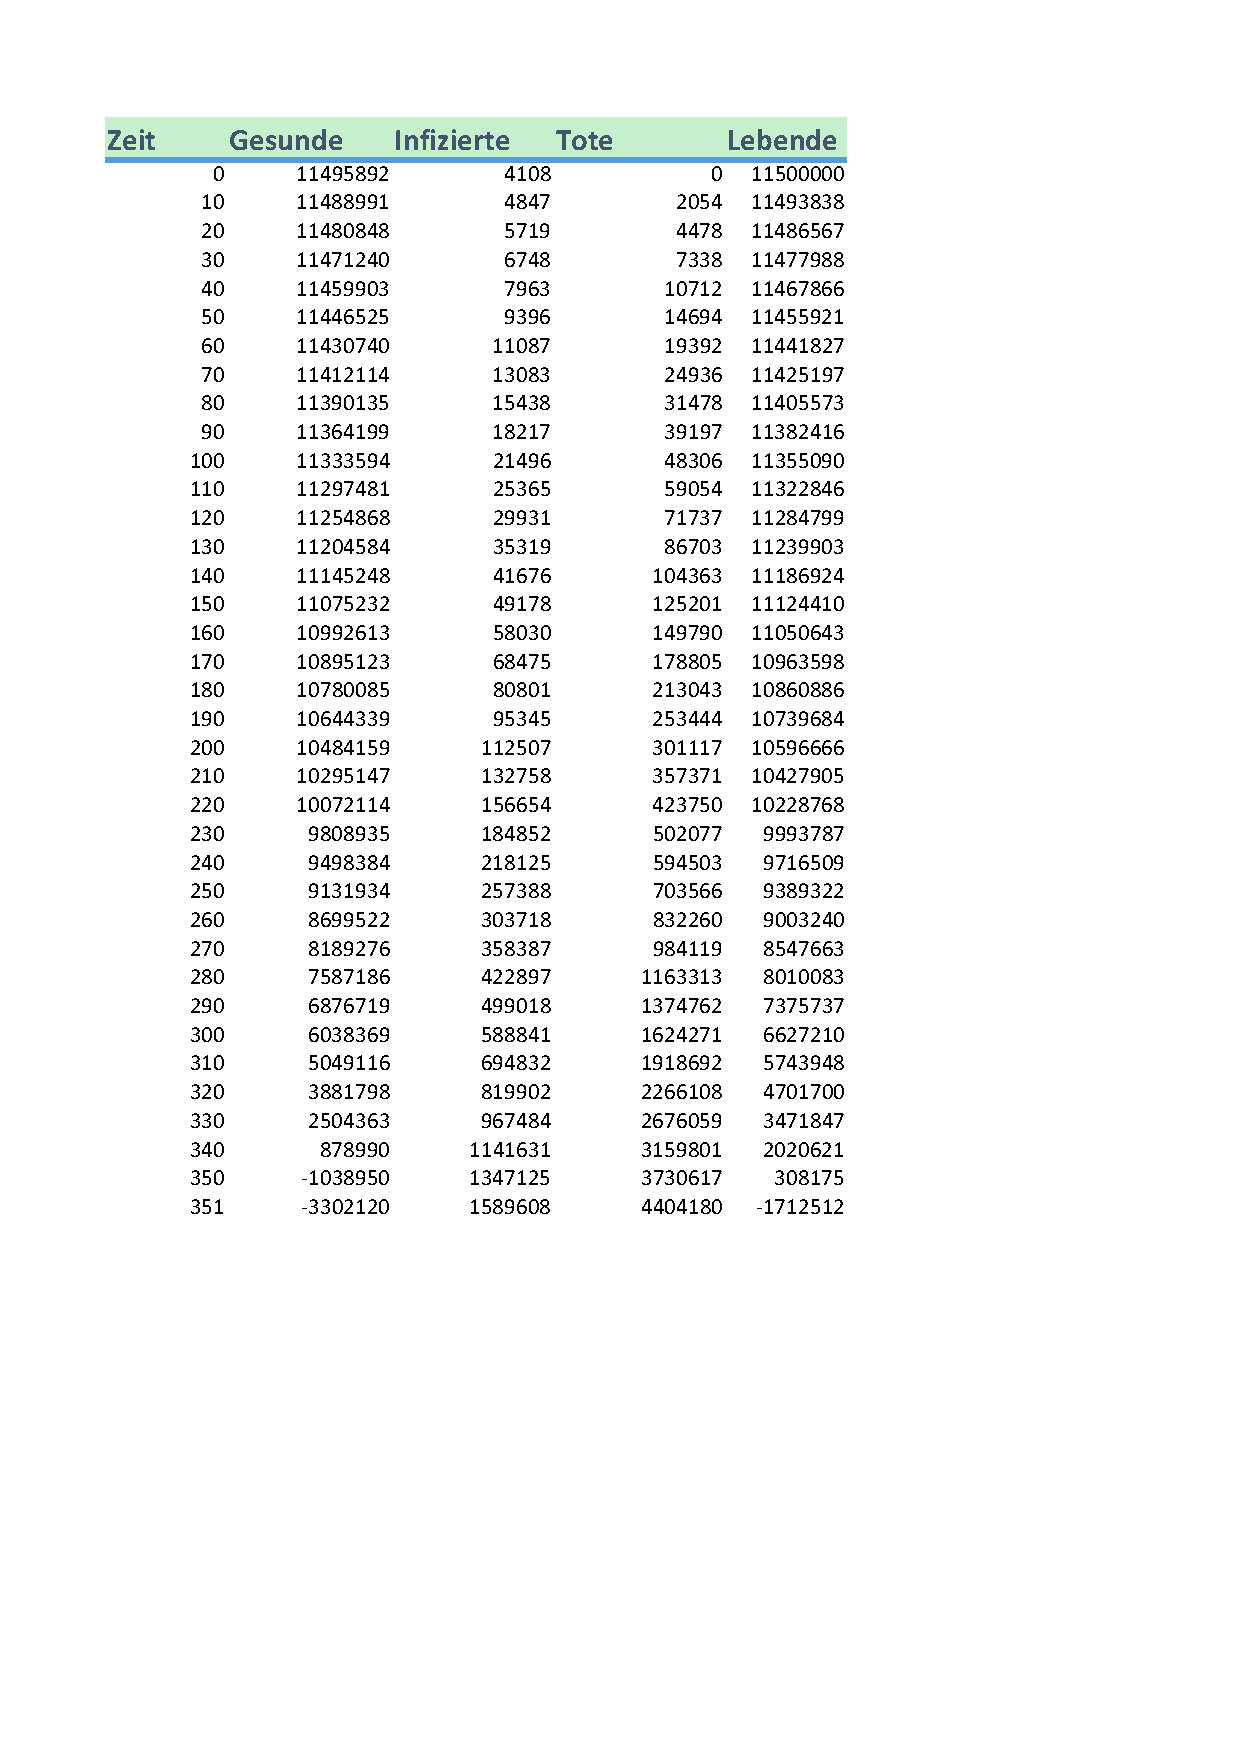
\includegraphics[width=\textwidth]{projekt/leistung_1_1}}\newpage
\noindent\frame{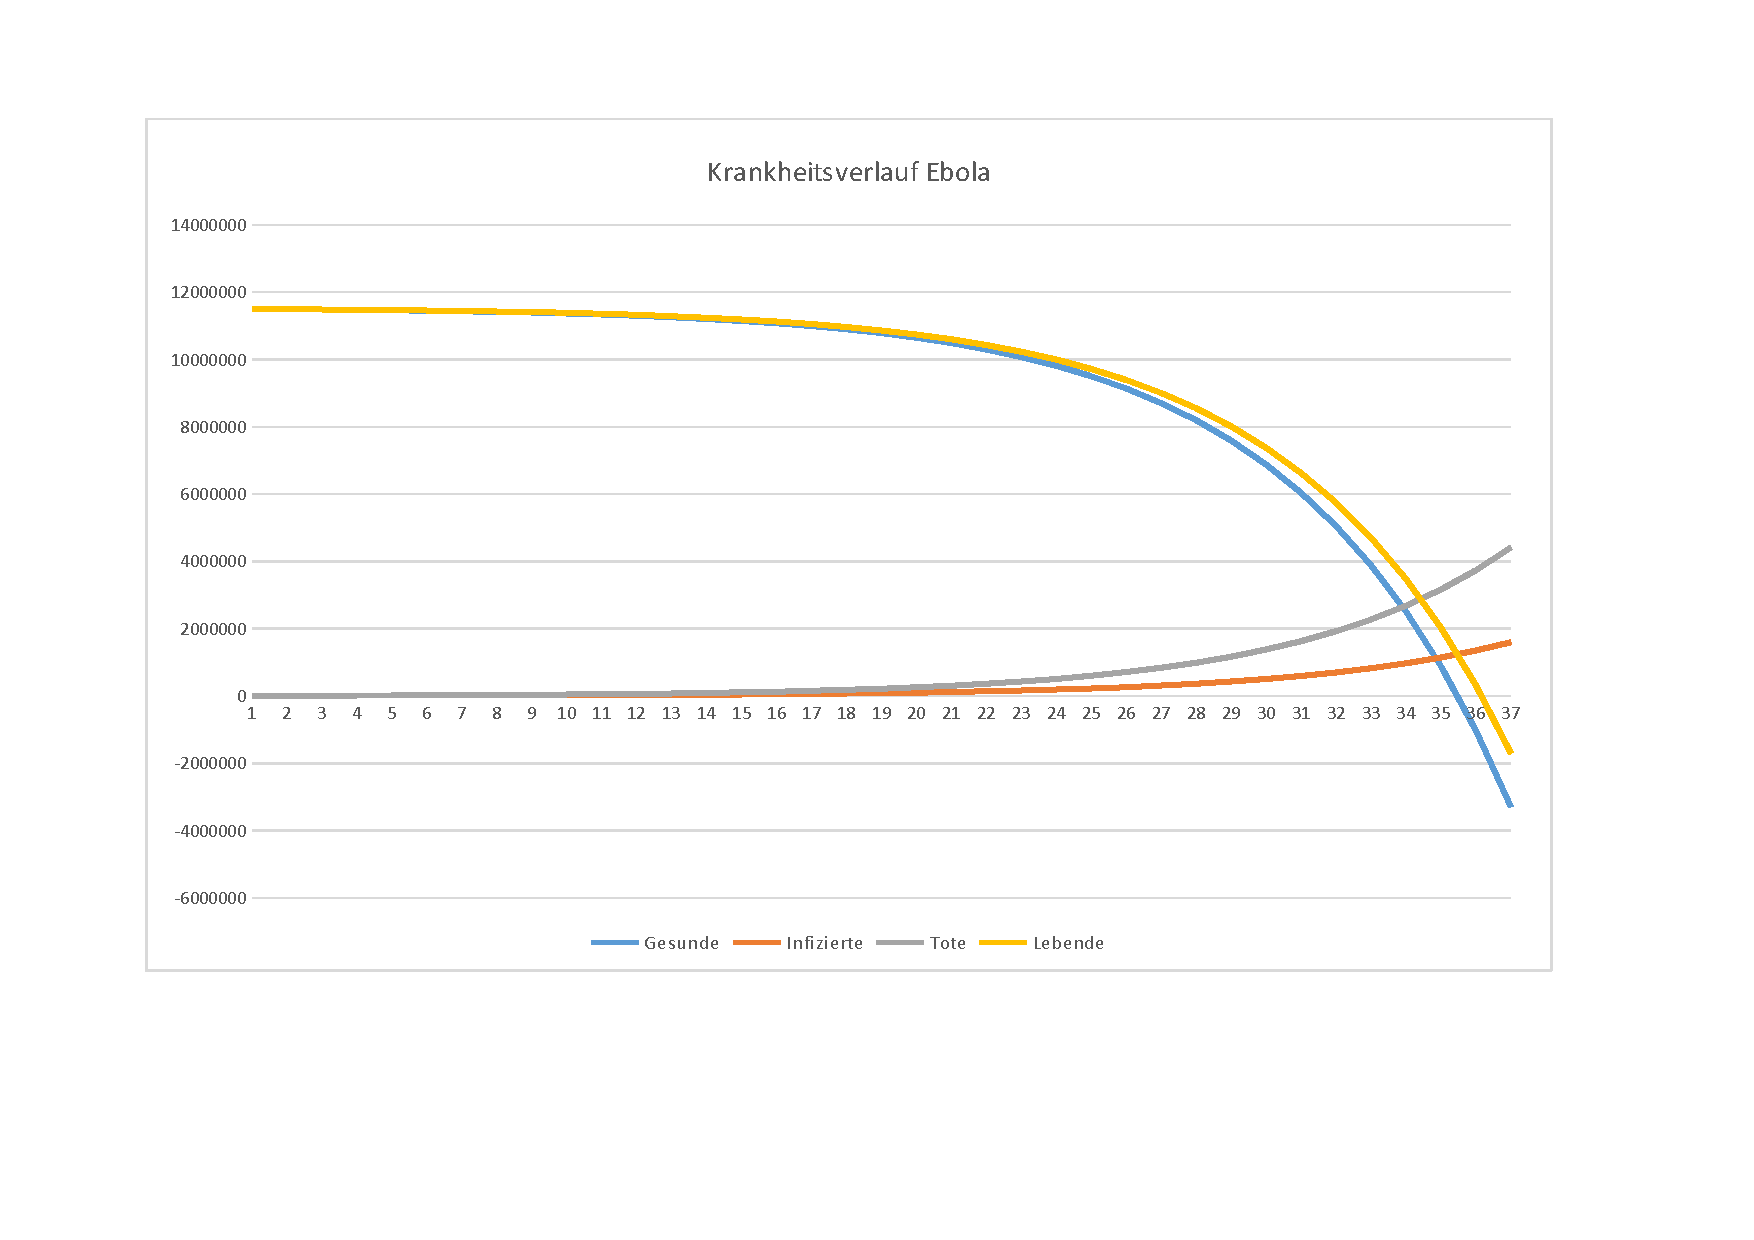
\includegraphics[width=\textwidth]{projekt/leistung_1_2}}\newpage
Alle Produkte der Schülergruppen entsprechen mindestens dem Erwartungshorizont. Das oben angeführte Beispiel zeigt aber zusätzlich ein Schülerprodukt, das die Erwartungen weit übertrifft. Darin zeigt sich, dass eine Differenzierung der Aufgabenstellungen dringend notwendig ist. Einige Gruppen benötigten viel Zeit um sich mit dem Tabellenkalkulationsprogramm vertraut zu machen, während das obige Beispiel zeigt, dass es auch Gruppen gab die nach Bearbeitung der Aufgabe noch die Zeit hatten, einen Graphen zu plotten der den Verlauf nochmal verdeutlicht.  

\subsubsection{Reflexion der Stunde}
Die Schülerinnen und Schüler haben zum Teil neue Funktionen der Tabellenkalkulationsprogramme kennen gelernt. Zudem haben sie Grundlegende Vorgänge der Modellbildung genutzt und eigenständig Modelle aufgestellt. In diesem Zusammenhang wurde auch das Aufstellen von Funktionen wiederholt und vertieft.\\
Die Schülerbeteiligung war sehr hoch, ohne Anstoß durch die Lehrperson haben sie die Vorschläge der Gruppen gemeinsam korrigiert und in einem angenehmen Klima fachlich diskutiert. Zusätzlich wurden schon früh Verbesserungsvorschläge für das Modell angebracht.\\
Da die Klasse unbekannt ist, war die Zusammensetzung in der Partnerarbeit nicht optimal. Wenn man die Lerngruppe besser kennt, könnte man Teams bilden, die sich gegenseitig unterstützen. Dadurch könnten die großen Unterschiede im Zeitbedarf angepasst werden.\\
Ist dies jedoch nicht möglich, sollte es Aufgaben geben, die die besonders schnellen zusätzlich erledigen können.\\
Statt der beiden Simulationen konnten die Gruppen in der Stunde nur eine Simulation durchführen. Dies ist jedoch von Vorteil für die nächste Sitzung, da an diesem Tag acht von siebzehn Schülern fehlten.\\
Daher wird in der nächsten Stunde eine größere Wiederholung stattfinden. Von allen Gruppen wird dann lediglich die zweite Simulation durchgeführt und die dritte Simulation steht für die besonders schnellen Schülerinnen und Schüler zur Verfügung. 
\newpage
\subsection{Projektstunde 3 \& 4}\ellen
\subsubsection{Bemerkungen zur Lerngruppe}
Durch Beobachtungen in der ersten und zweiten Stunde konnte festgestellt werden, dass es große Unterschiede in der Leistungsfähigkeit am Computer zwischen den Schülerinnen und Schülern gibt. Die Leistungsbereitschaft und Mitarbeit ist jedoch bei nahezu allen überdurchschnittlich hoch.\\ Zudem wirkt die Lerngruppe sehr interessiert am Thema, sodass eigenständige Erarbeitung über die Unterrichtszeit hinaus erwartet werden kann.\\
  Insgesamt arbeiten die Schülerinnen und Schüler sehr selbstständig und konzentriert. 
\subsubsection{Methodische Überlegungen}
Zunächst sollte eine Wiederholung der letzten Stunden vorgenommen werden, da nahezu die Hälfte der Schülerinnen und Schüler nicht anwesend war.\\
Dabei sollen die Schülerinnen und Schüler selbstständig erzählen, was behandelt wurde. Parallel dazu wird eine Skizze an der Tafel angefertigt. Diese zeigt schemenhaft das erarbeitete Modell. Somit erhalten alle Schülerinnen und Schüler einen Überblick und lernen eine Möglichkeit um Modelle darzustellen. Zusätzlich soll diese Darstellung im weiteren Verlauf der Unterrichtseinheit häufiger verwendet werden.\\
Da die Lerngruppe eher fortgeschritten ist, wird in diesem Fall auf eine explizite Einführung des Schemas verzichtet. Dies wäre alternativ auch möglich, ist jedoch an dieser Stelle noch nicht notwendig. Statt dessen wird beobachtet, ob die Lerngruppe die Art der Darstellung selbstständig übernimmt. Falls dies nicht der Fall ist, kann sie später explizit eingeübt werden.\\
Im weiteren Verlauf der Stunde sollen die Schülerinnen und Schüler ihr Modell mit neuen Informationen überarbeiten. Dadurch soll gewährleistet werden, dass sie zumindest zweimal den Modellierungskreislauf durchlaufen sind. Durch die Vorgabe der Informationen wird Zeit eingespart und die Vergleichbarkeit wird gewährleistet. Alternativ ist es auch möglich, der Lerngruppe freizustellen wie sie ihre Modelle verbessern möchten. Dadurch würde die Selbstständigkeit der Schülerinnen und Schüler gestärkt, ihre Motivation könnte zusätzlich erhöht werden, da sie ihre eigenen Vorstellungen umsetzen könnten und schließlich könnte später eine Diskussion über die verschiedenen Modelle geführt werden.\\
Zudem wird hier darauf verzichtet, das Modell zunächst alleine zu entwickeln. Dies liegt daran, dass die Hälfte des Kurses einen erheblichen Vorteil hätte, da diese bereits ein Modell entwickelt haben, das lediglich erweitert werden muss. Um eine gleichmäßige Beanspruchung zu gewährleisten, werden die Paare so gebildet, dass immer eine Person, die in den ersten beiden Stunden anwesend war mit einer Person zusammen arbeitet, die nicht anwesend war.\\
Da die Selbstständigkeit der Lerngruppe jedoch bereits sehr hoch ist und durch das große Interesse das Risiko besteht, dass die Modelle zu komplex werden, wird hier auf diese zusätzliche Freiheit verzichtet.\\
Danach werden die Ergebnisse wieder verglichen. Dabei wird darauf geachtet, dass die Ergebnisse der Simulation in Prognosen für die Realität übersetzt werden.\\
Zuletzt wird gemeinsam mit der Lerngruppe ein Tafelbild über den Modellierungskreislauf erstellt. Durch die gemeinsame Erarbeitung sollen die Schülerinnen und Schüler das angewendete nochmals wiederholen und somit vertiefen.\\
Alternativ könnte man ein vorgefertigtes Tafelbild erstellen, welches dann lediglich mit den Schülerinnen und Schülern besprochen wird.

%\subsubsection{Verlaufsskizze}
\begin{landscape}
\subsubsection{Verlaufsskizze}
\noindent
\begin{tabular}{|C{0.3\textwidth}|L{0.8\textwidth}|L{0.4\textwidth}|}
\hline
Phase & Arbeitsauftrag & Sozialform\\
\hline\hline
Begrüßung & keine & Lehrervortrag\\
\hline
Einstieg & Wiederholung der letzten Stunde & Schülervorträge\\
\hline
Erarbeitungsphase (a) & Modell erweitern zur Simulation einer Ebola Epidemie & Partnerarbeit\\
\hline
Erarbeitungsphase (b) & Das neue Modell mit Hilfe von Tabellenkalkulationsprogramm umsetzen & Partnerarbeit\\
\hline
Reflexionsphase & Modelle der SuS werden vorgestellt und Stärken und Schwächen der Modelle besprochen & Schülervorträge + Diskussion\\
\hline
Zusatz & Mit weiteren Informationen und den Überlegungen aus der Diskussion wird das Modell verbessert und wieder eine Simulation durchgeführt & Partnerarbeit\\
\hline
\end{tabular}
\end{landscape}
\subsubsection{Materialien}
Als Material dient wieder das Informationsblatt aus den ersten beiden Stunden.
\subsubsection{Erwartungshorizont}
Es werden Formeln erwartet, die denen der ersten beiden Stunden entsprechen. Zudem werden ähnliche Tabellen erwartet.
\subsubsection{Schülerprodukte}
\subsubsection{Reflexion der Stunde}
Die Lernziele der Stunde wurden erreicht. Die Schülerinnen und Schüler waren in der Lage komplexere Formeln als in den ersten Stunden aufzustellen. Zudem konnten sie ihre Modelle wieder im Computer umsetzen und auch der Modellierungskreislauf schien ihnen ersichtlich zu sein.\\
Es war jedoch nicht genügend Zeit eingeplant um die Formeln der Schülerinnen und Schüler zu besprechen. Da die Aufgaben sehr offen gestellt waren, erarbeiteten die Schülerinnen und Schüler recht unterschiedliche Modelle. So hatte eine Gruppe die mittlere Überlebenswahrscheinlichkeit berechnet und diese in die Formeln eingesetzt, statt dauerhaft zwischen hospitalisierten und nicht hospitalisierten Patienten zu unterscheiden. Eine weitere Gruppe hat für die nicht hospitalisierten eine zusätzliche Klasse erstellt.\\
Man sollte also genügend Zeit einplanen, um verschiedene Modelle zu besprechen und möglicherweise Vor- und Nachteile der einzelnen zu erkennen.\\
Eine weitere Möglichkeit wäre an dieser Stelle auf eine Besprechung zu verzichten. Dann können die Schülerinnen und Schüler ihre Modelle testen und im Vergleich Vor- und Nachteile finden. \\

\newpage
\subsection{Projektstunde 5 \& 6}\steffen
\subsubsection{Bemerkungen zur Lerngruppe}
\subsubsection{Methodische Überlegungen}
\subsubsection{Verlaufsskizze}
\subsubsection{Materialien}
\subsubsection{Erwartungshorizont}
\subsubsection{Schülerprodukte}
\subsubsection{Reflexion der Stunde}